\section{Audio System}
\label{dmx_section}
Like every other I/O system in the engine, the audio is abstracted behind an interface. To fulfill \doom's core expectations such a system has to implement at least twenty functions covering SFX, Music, and also the Timer. Here are a few.\\
\par
 \begin{figure}[H]
\centering  
\begin{tabularx}{\textwidth}{ L{0.57}  L{1.43}}
  \toprule
  \textbf{Method} &  \textbf{Usage}\\

  \toprule 
  I\_StartupSound & Initialize Audio system, detect audio hardware\\
  I\_SetChannels & Set number of channels and sample rate\\
  \toprule 
   
I\_RegisterSong & Upload a music lump and get back an ID.\\
I\_SetMusicVolume & Self explanatory.\\
I\_PlaySong & Play Song\\
I\_PauseSong & ...hm, Pause Song\\
I\_ResumeSong & Mysterious function with unknown effects.\\
I\_StopSong & Maybe this array was not a good idea after all.\\
I\_UnRegisterSong & Free music using ID obtained in \cw{I\_RegisterSong}.\\




  \toprule 
I\_GetSfxLumpNum & Upload audio sample from WAD and return an ID.\\
I\_SetSfxVolume & If you read this, you are a real human being and a real hero.\\
I\_StartSound & Start playing SFX sample.\\
I\_StopSound & Stop playing SFX sample and free it.\\
I\_SoundIsPlaying & Test if SFX is playing.\\
I\_UpdateSoundParams & Set pitch, left/right position and volume.\\

  \toprule 
  
I\_StartupTimer & On DOS triggers audio system to hook into the Intel 8259 PIC. No-op on other platforms.\\
I\_ShutdownTimer & On DOS remove the hook.  No effect on other platforms.\\

   \toprule
\end{tabularx}
\caption{\doom{} audio system interface}
\end{figure}



On NextStep this system was never a problem since only the timer function had to be implemented. On the PC side however the game engine had to have sound effects and music. One difficulty was the fragmentation of the sound card market which had increased exponentially since Wolfenstein 3D. The previous title required tremendous effort to support four sound sources. Two years later there were more than fifteen chips available, all with different types of bugs, quirks and technologies.\\
\par
To make things worse, the departure of Jason Blochowiak had left id Software with both a shortage of expertise and enthusiasm toward audio. They solved the problem by throwing money at it and licensed the DMX library. For the price of its license, the library authored by Paul J. Radek offered an all-in-one audio solution. With support for all major sound cards, convenient means to detect them, support of many sound and music formats, and an easy way to integrate with any game engine, DMX was a perfect fit which undoubtedly saved id several months of development.





The abstraction layer provided by DMX was a colossal task. The comment before the function in charge of detecting the hardware leaves no ambiguity to how much of a burden it was to tackle this problem.\\
\par
\ccode{whypcssucks.c}\\
\par
With DMX backing the sound system, ten audio chipsets were supported.\\
\par
\ccode{cardenum_t.c}\\
\par
Running on an operating system supporting neither threads nor processes, there was seemingly not way to generate both the video and the audio output simultaneously. An attentive reader will have noticed the hardware section mentioning two chipsets i8259 (Programmable Interrupt Controller: PIC) and i8254 a (Programmable Interval Timers: PIT). Together they can be set up to interrupt the engine execution and call into DMX routine\footnote{The way PIC and PIT interact is extensively detailed in "Game Engine Black Book: Wolfesntein 3D".}.\\
\par
Upon initialization, DMX installs itself as an interrupt handler via the PIC and the PIT in order to be called at 140Hz. Upon awakening DMX interrupt handler takes care of feeding the audio device with music and sound effect data provided by the engine.\\
\par
 Since the was no other "high precision" timer on the machine, DMX was also in charge of generating the game's heartbeat via a variable counter called \cw{ticcount}.
\par


\scaleddrawing{1}{sound_manager_architecture}{DMX architecture}
With such an architecture there are two systems executing pseudo-concurrently but the audio has more constraints than video. When an interrupt is triggered, DMX has only a few milliseconds to refill the sound card buffers and go back to sleep. If DMX is too slow, it can delay video rendering or mask other interrupts.\\
\par
 This explains why audio assets allocation get a special treatment in the zone allocator. The audio system has no time to recover from a memory miss (nor could it since it has no access to the wad or memory allocator). Audio data must be ready at all time it is needed.

\subsubsection{Audio Data: Formats and Lumps}
The wad archive contains hundreds of lumps of five types to feed to DMX. \cw{DP*} lumps are for PC Speaker Sound Effects, \cw{DS*} lumps are for PCM Sound Effects, \cw{D\_*} lumps are for musics. There is also a \cw{GENMIDI} lump, and one \cw{DMXGUS} lump detailed later.\\
\par
PC Speaker audio was meant for PCs without a sound card. The PC Speaker was capable of square waves and meant to emit boot-up diagnostic noises. \doom{} found ways to make it generate something less irritating by changing the square frequency every 1/140th of a second\footnote{PC Speaker are detailed in "Game Engine Black Book: Wolfenstein 3D".}. The data rate is one byte per 1/140th of a second, describing what square-wave frequency to set.\\
\par
 Digitized audio samples used in \doom{} are 8-bit, 11025 Hz, mono PCM streams. PCM is a simple audio format which requires little explanation. Each byte in the stream is a moment in time that describes the amplitude of a waveform and indicates where the speaker cone should be positioned. The sound card simply translates the byte into a voltage to the magnet driving the cone position, which happens at a rate of 11025 times per second.\\
\par
Music data was stored in \cw{MUS}, a format similar to standard MIDI only slightly more compact. The format allows eight channels for instruments and a ninth one for the drums. The MUS format describes, for each channel, a series of precisely timed events that specify which instrument should play a note and at what pitch. Note that MUS only describes what to do and when, not how to do it. Each channel refers to the note of an instrument , the latter of is described elsewhere in a data structure known as the "instrument bank".\\
\par
The instrument bank is stored in the \cw{GENMIDI} lump. It is aimed at SoundBlaster compatible sound cards based on an OPL2 chip synthesizing music with Frequency Modulation. The lump describes how to play the note of each instruments in the MIDI repertoire. There are 175 entries in \cw{GENMIDI}, one for each of the 128 standard General MIDI instruments and 47 percussion effects. Each entries describes how to setup a channel in order to emulate an instrument. A channel is made of two cells, where one cell is used as carrier and the other as modulator. For each cell, attack, decay, sustain, release, harmonic, and waveforms can be selected by the musician\footnote{Source: "The dark and forgotten art of GENMIDI" }. Instrument banks were 90s musician's "secret sauce" and \doom's were famous for being excellent.\\
\par
The \cw{DMXGUS} lump fulfilled the same goal as \cw{GENMIDI} but for the Gravis Ultrasound card. It enabled the GUS to play MUS music notes, not with an FM synthesizer but with the PCM samples provided with GUS drivers. It is a simple lump mapping MIDI instruments to GUS instruments with special rules for RAM allocation depending on the amount of RAM installed on the board (256KiB, 512KiB, 768KiB, and 1024KiB).\pagebreak



Dealing with so much complexity proved difficult for DMX. Some of the craziness Paul Radek had to deal with surfaced in a post on \cw{vogons.org}\footnote{Forum thread: "Gravis Ultrasound - Hardware Mixing Game List".}.\\





\fq{All of the sound effects are now mixed in software, rather than on the GUS hardware. Why, you ask? Because of several reasons. First, is that the GF1 chip has a minimal ramp time that is much to long for very sharp effects. Second, because loading of the MUSIC patches uses all of the GUS memory, I had to DMA all eight sound effects to the card when played. This intern exposed a bug in the GF1 chip that Gravis did not find until my code started to beat on it. The bug would cause the bus to freeze and any program with it. The workaround is to keep DMA activities to a minimum by mixing in software and transferring only 1 channel to the GUS. But since the GF1 can't support auto-initialize DMA, and because the only way to play interleaved data on the card is to set two voices pointing into a single patch and setting the frequency so the every other sample is skipped, you don't get the benefit of sample smoothing from the GF1.\\
\par
Sorry, but that's the way it has to be :(\\
}
{Paul Radek, Digital Expressions, Inc.}\\
\par

The library evolved during the development of \doom. Sometimes API changes introduced bugs. Gravis UltraSound support was broken with v1.666. Support for Audio Spectrum was also broken so the card had to fallback on (poor) SoundBlaster emulation\footnote{Source: John Romero post on \cw{alt.games.doom}.}.\\
\par
The problem was partly due to poor API practices on DMX side and partly because of hasty adjustments on id Software part. Most issues were ultimately fixed except for one major bug which made it to customers. The engine was originally supposed to emit sounds at random pitch to avoid monotony. To this effect, DMX function \cw{SFX\_PlayPatch} was used.\\
\par
\ccode{dmx_before.c}





It originally worked as intended but then DMX API was modified in an uncanny way. It may not be immediately apparent but function \cw{SFX\_PlayPatch} parameters have been swapped.\\
\par
\ccode{dmx_after.c}\\
\par
 Invocation sites were never adjusted and the game shipped without random pitch feature, instead randomly balancing sound between the left and right channel.\\
\par
\ccode{I_StartSound.c}\\
\par
In retrospect John Carmack regretted using DMX because it led to issues when open sourcing the game engine (it is unknown if Paul Radek was unwilling to open source DMX or if id software was unwilling to negotiate with him).\\
\par
\fq{
Our biggest mistake during DOOM development was the contracting of an  
outside party to do dos sound drivers.  Because we had this black box  
functionality coming, I didn't simulate it under NS.  BAAAAAD mistake.   
All future work will be entirely developed under NS, with only DMA  
buffer flipping being the hardware layer.  We will probably also run  
midi under NS for music (which will be dynamically tuned to the game  
situation in Quake).}{John Carmack}\\
\par
Additionally, one can still find archived usenet posts from \cw{alt.games.doom} where John Romero comments suggest that the relationship between Radek and id software was suffering as the game neared its released date\footnote{Source: John Romero post on \cw{alt.games.doom}.}. Since tone was less than cordial, it is left as an exercise to the reader if they want to dig these posts out. I do not recommend it.
% \par
% \fq{Hey, everybody!  Thanks a lot for downloading DOOM II -- that's really "cool".   
% We love it when we send evaluation copies to magazine editors and some piece of  
% shit uploads the thing.  The DOOM II out there is the master copy we sent to GT  
% Interactive, our distributor.  If your GUS sound doesn't work, it's probably  
% because your IRQ is > 7.  Our sound code dork broke part of the sound support  
% while he was "expanding" it, so IRQs > 7 don't work, Pro Audio Spectrum owners  
% now have to run their SB-emulation driver (no more native support), etc.  The  
% sound guy is a real shithead.  All these fuckups are in v1.666 as well --  
% sorry.  We have NO time to wait and hope that sound-dork fixes these problems,  
% as he's demonstrated in the past year and a half that he's incompetent.}{John Romero (alt.games.doom)}



\section{Sound Propagation}
How well enemies react to sounds makes a tremendous impact on how smart the A.I is perceived. id Software made sure sound propagation was realistic. When a shot is fired in a sector, a flood fill algorithm propagates the noise.\\
\par
\ccode{P_RecursiveSound.c}\\

\begin{wrapfigure}[10]{r}{0.48\textwidth}
\centering
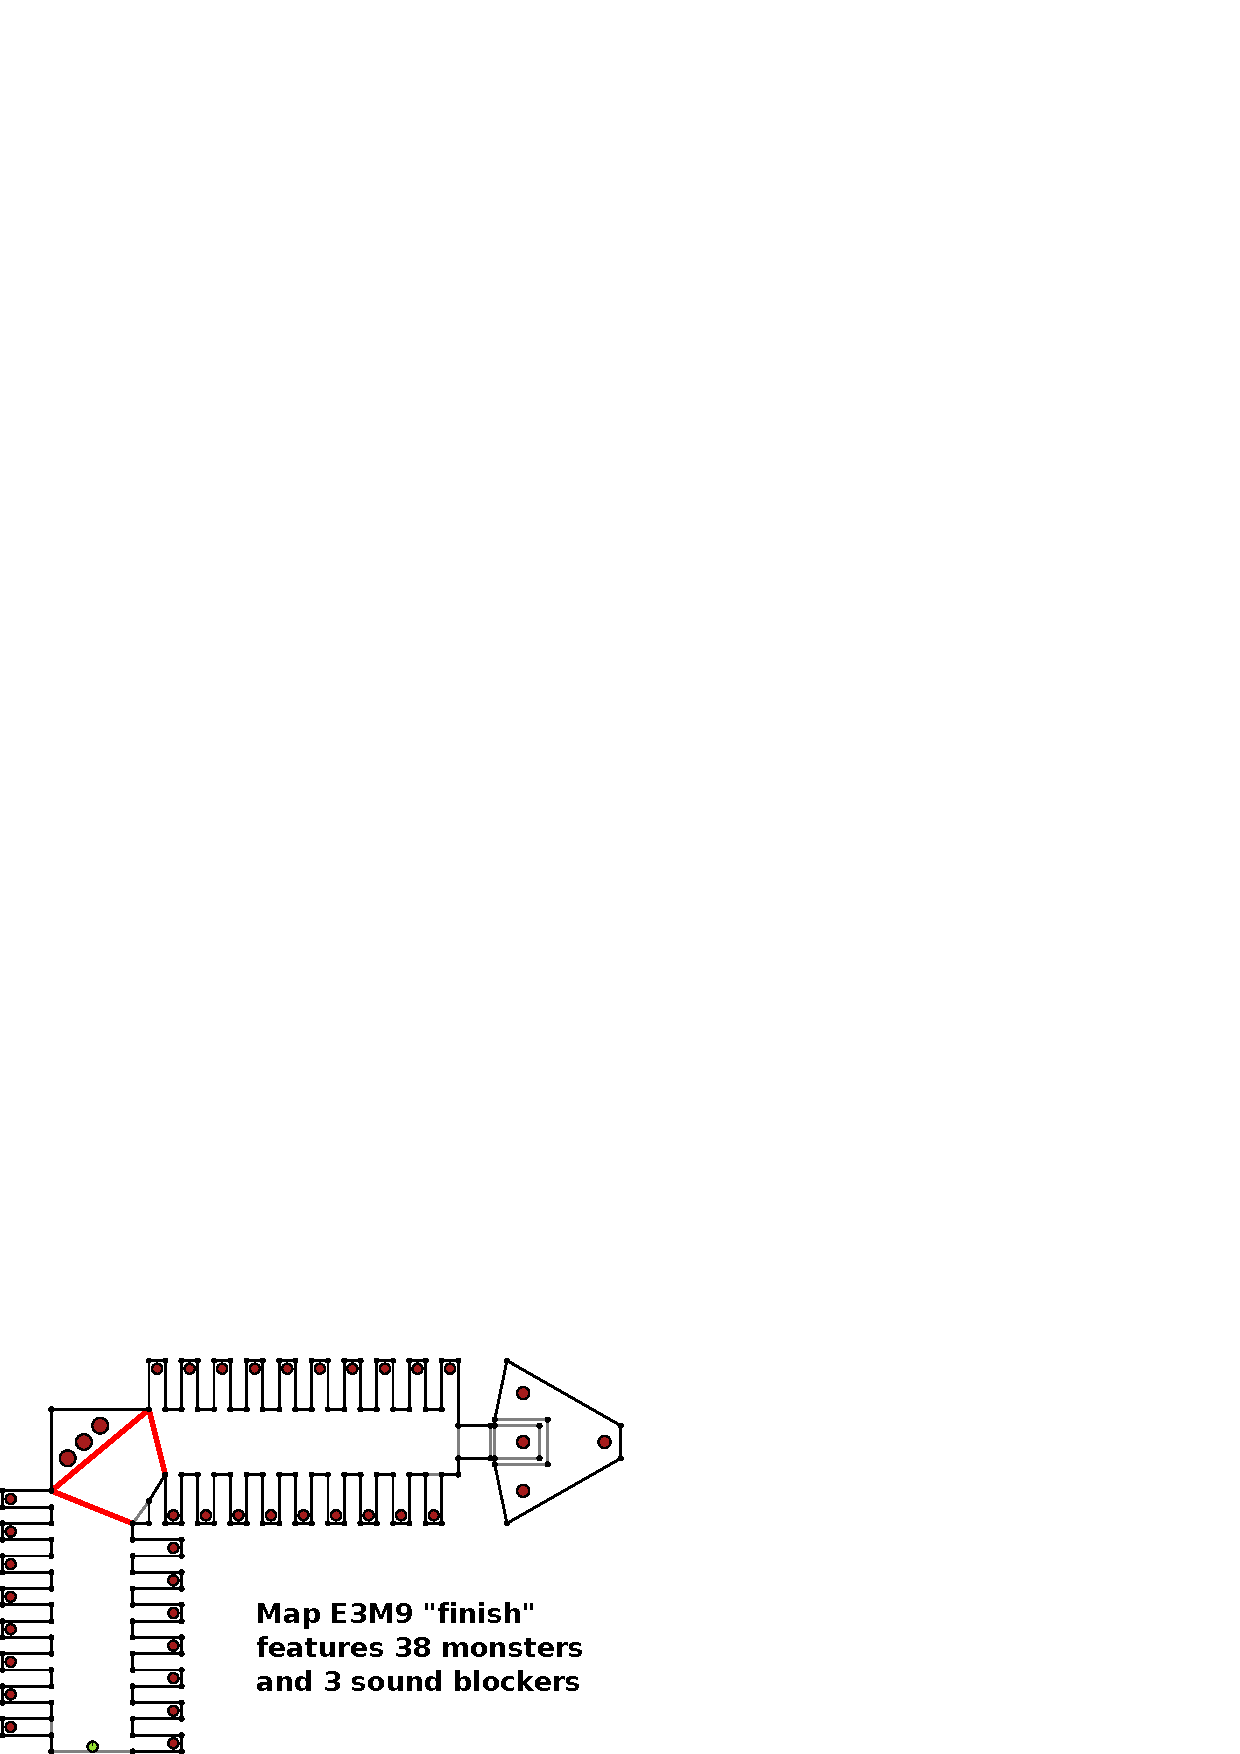
\includegraphics[width=.48\textwidth]{drawings/sound_blockers.pdf}
\end{wrapfigure}
  The sectors/portals format is leveraged. Starting in the current player sector and flood-filling into adjacent sectors via portals (two-sided lines). Sound is stopped when either a door is encountered or when two "sound blockers" lines have been crossed. In map E3M9 featuring a section with 38 monsters the A.I cost is lowered with three (red) line blockers which keeps some monsters dormant.\\
\par
Notice how function \cw{P\_RecursiveSound} mentions "waking up all monsters" but never iterates over the list of things in the level. This is a speed-up trick aimed at avoiding an expensive search to find all monsters to be awakened in each sector. Monsters always look up for the current sector's \cw{soundtarget} to pick a target. By simply assigning a value to \cw{sec->soundtarget}, all monsters in \cw{sec} automatically acquire the same target.\\
\par
\rawdrawing{E1M1_audio_sections}
\par
\subsubsection{Ambushing}
Map designers wanted to have sneaky monsters whom could hide and wait to jump on a player. This is achieved via a MF\_AMBUSH tag assigned to monsters. It doesn't make monsters deaf, it only makes them not seek the player until they make visual contact.


\subsubsection{Super Ambushing}
Sound propagation was used in a inventive way for map E1M9 super ambush.  The designers wanted the player to be swarmed with monsters teleporting, seemingly from an hellish dimension, as soon as doomguy walked through the center of a pentagram.\\
\par
 But without a scripting language available that was next to impossible to implement. As we'll see in the A.I section, monsters are state machines able to do only three things: Stay dormant, pursue a target, and when they bump into walls and things, change direction.\\
\par
\begin{wrapfigure}[24]{r}{0.52\textwidth}
\centering
\includegraphics[width=.52\textwidth]{drawings/e1m9_sides.pdf}
\end{wrapfigure}

\par

To achieve the effect anyway, they created an unaccessible "monster pool" room next to where they wanted the super ambush and filled it with monsters (red circles in the drawing). In the right bottom of the hidden room, they place a teleporter, protected by walls.\\
\par
Then they created a very tiny pipe to allow sound to flow between rooms so when the player was fighting in his room, all monsters in the "pool" room would be awakened and try to reach the player. Without a way to get there (the monsters at too big to go through the pipe and also the pipe is at ceiling level) monsters started to run in circle with a tendency to go toward the player location (south-east).\\
\par
The last piece of the super ambush trap was to have four tripwires around the center of the "pentagram which lowered the walls around the teleporter. A bait was placed on it (such a lots of health and ammunitions) to make sure the player would go there.\\
\par

As soon as the player walked on the trigger in the "star" room, the walls around the teleporter lowered, monsters moved toward it and swarmed the player's room. \\
\par
\trivia{Comments in the code suggest that monsters screaming awaken other monsters but it is not the case. It is unknown why this feature was cut. Maybe it was too buggy or too expensive.}







John Romero himself described how they called these sound conduits, "pipes".\\
\par
\fq{We used sound zones in Wolfenstein 3D as another way to alert enemies to your presence. In DOOM, we did the same thing but used sectors as the conduits of audio travel. This was a really important part of making the game scary, as sound could leak all over the place and alert demons. You might see lots of little sector pipes that connect sectors together just to alert monsters-sectors that you'd never see because we put them way up high in the corner of a room. So, we paid a lot of attention to the sound flooding.}{John Romero, p29 in Scarydarkfast}\\
\par
The audio pipe in E1M9 super ambush is so well hidden in the ceiling that it is very hard to notice it with the vanilla engine. The room is dark and in the distance, the tiny black rectangle blends in the obscurity. Opening the map with an editor such as Slade which allows to look up and down reveals the stratagem.\\
\par
\cfullimage{sound_conduit.png}{}
\par
In figure \ref{sound_conduit.png} the audio conduit is visible in the upper right corner.
% In figure \ref{sound_conduit.png}, the audio conduit to awaken the monsters and make them go to the teleporter is visible in the upper right corner (screenshot done with the amazing Slade3 Node Editor).
